% Created: Enze Chen, July 2017
% Last edited: Enze Chen, December 2017
%
% Chapter 9 of the MSE 142 coursereader. This chapter summarizes the content of the course, and provides some further topics of exploration. Some other related courses in the materials science curriculum are also discussed.

% Uncomment the following three lines and last line to individually compile this chapter
%\documentclass[12pt, english]{book}
%\usepackage{142crstyle}
%\begin{document}

\chapter{What's Next?} \label{ch:next}
%{ \doublespacing 
\begin{figure}[!h]
	\centering
	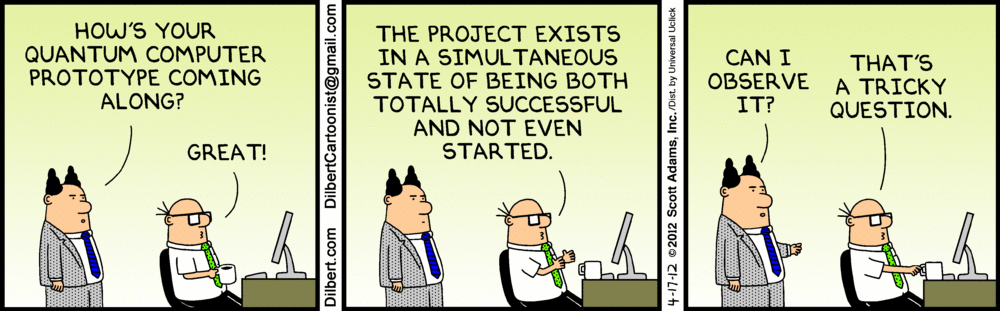
\includegraphics[width=0.9\linewidth]{dilbert-quantum}
	\caption{Image courtesy of \href{http://dilbert.com/strip/2012-04-17}{Dilbert}.}
\end{figure}
Congratulations! It's been a long quarter, and you should feel proud for everything you've accomplished in this class. This short, final chapter is meant to summarize some of the key concepts and learning objectives from this course, and provide motivation for where to go from here. 

\section[Recap]{Recap of content and learning objectives}
My goal with this course was to provide a basic introduction to the world of quantum mechanics, which is an immensely rich, exceedingly vast, and nefariously complicated subject. Along the way, I hope you felt sufficiently challenged to think in abstract and quantitative ways that often broke with intuition. Recall that we began with the Stern-Gerlach experiment as a shock treatment that led into a narrative of the development of quantum theory. Although many of these ideas are almost a century old, they are still hotly debated and continue to feature in scientific discoveries! \par 

As you've seen, just about every problem in quantum mechanics involves formulating some version of the \Sch\ equation and then solving it, so the \Sch\ equation was a natural place for us to start. We introduced the concept of a wave function to represent a quantum state and used the statistical interpretation to arrive at the probability density function. Then, we saw our first and perhaps simplest quantum mechanical system, which was that of the particle in a box. Using this simple but powerful model, we solved the time-independent \Sch\ equation and arrived at the quantization of energy levels, which was just the first of many surprising behaviors at the nanoscale. \par 

From there, we experimented with different types of rectangular potential barriers, and saw how it was possible for a particle to tunnel through a potential barrier that it could not classically surmount. This is another phenomenon that is only observed at the quantum scale, but appears in a wide variety of contexts. In particular, we used it to analyze the Kronig-Penney model for periodic potentials, and surprisingly we found entire bands of energies that were forbidden for electrons. \par 

In order to analyze the quantum harmonic oscillator, we went one step further to parabolic potentials and used the formalism of operators to solve this instance of the \Sch\ equation. Those concepts provided the foundations for quantum field theory, which we developed to explain second quantization and phonons. Finally, we introduced a time-dependent term into the Hamiltonian and developed the framework of time-dependent perturbation theory to model the interaction of matter with electromagnetic fields. \par 

We have learned \emph{a ton} since this course first started ten weeks ago! You now have basic fluency in the language of quantum mechanics---which many schools don't teach until the graduate level---and you're now better equipped to solve problems that originate from the nanoscale. There was quite a bit of advanced mathematics in this course, and I hope you saw those as tools to facilitate learning rather than barriers to approaching the subject.

In addition to the theory, another major goal of this course was to show the application of quantum mechanics in nanoscale devices and physical systems, many of which you might encounter in your later studies. My attempt to match an application to the topic of each chapter was both to demonstrate the utility of the knowledge and strengthen your understanding. Quantum mechanics is truly ubiquitous, and focusing only on the theory would miss out on this exciting opportunity to demonstrate its manifestations in the real world, which is important for everyone to understand, especially materials scientists. From devices like the laser and the scanning tunneling microscope to particles like quantum dots and phonons, I hope you had as much fun learning about the applications as I had sharing them.

%%%%%%%%%%%%%%%%%%%%%%%%%%%%%%%%%%%%%%%%%%%%%%%%%%%%%%%%%%%%%%%%%%%%%%%%%%%%%%%%

\section{Further topics} \label{sec:further}
As I mentioned just now, this course serves only as a brief introduction to quantum mechanics---there's so much more left to explore! Because we surveyed a wide variety of topics, you're well-prepared for further studies in this field should you choose to do so. A non-exhaustive list of interesting and important topics include:

\begin{itemize}
\item \textbf{Quantum entanglement}. This physical phenomenon occurs when groups of particles have quantum states that cannot be described independently of the states of other particles. We saw this in the case of the quantum eraser when knowing the state of one photon allowed us to immediately know the state of the coupled pair. This strange coupling effect that holds across both space and time shocked the physics community when it was first proposed and it was dubbed ``spooky action at a distance'' by none other than Einstein himself.\footnote{Check out the following article by L. Sanders, \href{https://www.sciencenews.org/article/everyday-entanglement}{\emph{Science News}} \textbf{178}, 11 (2010).}

\item \textbf{Hydrogen atom}. The list of quantum mechanical systems with analytical solutions is short,\footnote{See \href{https://en.wikipedia.org/wiki/List_of_quantum-mechanical_systems_with_analytical_solutions}{Wikipedia} for a list of solvable systems.} but it notably features the hydrogen atom, making this a great model for developing quantum theory. Analyzing the hydrogen atom gives one a better understanding of the spin and angular momentum operators, multi-particle behavior, and quantization of energy levels where the spacing gets successively \emph{smaller} with increasing energy.

\item \textbf{Dirac equation}. Some of the finer details regarding the hydrogen atom can only be solved with this equation developed by Paul Dirac, which also implies the existence of antimatter. It combines elements of quantum mechanics and special relativity, and should be approachable after our introduction to QFT.

\item \textbf{Quantum computing}. This field studies the performance of quantum computers by leveraging superposition and entanglement to perform calculations using quantum bits (qubits). Unlike regular bits, which have a value of 0 \emph{or} 1, qubits can exist in a superposition state of both 0 \emph{and} 1. Though quantum computers are still in their infancy, they may be able to solve problems that are unfeasible on classical computers and even crack state-of-the-art encryption techniques.\footnote{For some general reading on quantum computing and security, see N. Kobie, \href{http://www.wired.co.uk/article/quantum-computers-quantum-security-encryption}{\emph{Wired}}, 2016.}
\end{itemize}

%%%%%%%%%%%%%%%%%%%%%%%%%%%%%%%%%%%%%%%%%%%%%%%%%%%%%%%%%%%%%%%%%%%%%%%%%%%%%%%%

\section{Coursework}
There are also some really great courses here at Stanford that build on top of this course, covering both theoretical and applied concepts. \par 

\begin{itemize}
	\item \textbf{MATSCI 195} (with Jennifer Dionne) is a graduate-level course that takes many of the concepts in this course and applies them to waves and diffraction. You will definitely see a lot more of the math surrounding Fourier transforms, dispersion relations, and phonons.
	
	\item \textbf{MATSCI 152} (with Jennifer Dionne) is another undergraduate-level course that applies quantum mechanics to electronic materials. You will learn a lot more about band gaps and semiconductors as well as electron transport through solids. \textbf{MATSCI 199} (with Mark Brongersma) is a graduate-level course that covers similar topics as 152 but with greater depth and rigor.
	
	\item \textbf{MATSCI 331} (with Evan Reed) is a graduate-level course that focuses on using numerical computation to solve quantum mechanical problems. You will use computational methods to compute the electronic and optical properties of various interfaces and nanostructures.
	
	\item I do not have knowledge of specific offerings in other departments, but the ubiquitous nature of quantum mechanics means that there are plenty of courses in Applied Physics (APPPHYS), Physics (PHYSICS), Electrical Engineering (EE), and Chemistry (CHEM) that touch upon these concepts, and it's good for students to get exposure to different schools of thinking.	
\end{itemize}

%} % for doublespacing